\documentclass[crop,tikz, class=scrreprt, 8pt]{standalone} 
\usepackage[utf8]{inputenc} 
\usepackage[T1]{fontenc} 
\usepackage{xcolor} 
\usepackage[english]{babel} 
\usepackage[bottom]{footmisc} 
\usepackage{listings} 
\usepackage{pgfplots} 
\usepackage{amssymb}
%\usepackage{helvet} 
\usetikzlibrary{shapes.arrows, fadings}
\usepackage[eulergreek]{sansmath} 
\pgfplotsset{tick label style = {font=\sansmath\sffamily},every axis label/.append style={font=\sffamily\sffamily}} 
\pgfplotsset{compat=1.14} 
\usepackage{pgfplotstable} 
\pdfminorversion=5 
\pdfcompresslevel=9 
\pdfobjcompresslevel=3 
\clubpenalty10000 
\widowpenalty10000 
\displaywidowpenalty=10000 
\usepackage{emptypage} 
\usetikzlibrary{snakes}

\usepackage{transparent}

\usepackage{mathtools}
%
\DeclarePairedDelimiter\bra{\langle}{\rvert}
\DeclarePairedDelimiter\ket{\lvert}{\rangle}
\DeclarePairedDelimiterX\braket[2]{\langle}{\rangle}{#1 \delimsize\vert #2}

\tikzfading[name=fade left,
  right color=transparent!0, left color=transparent!100]
  
\usetikzlibrary{calc,fadings}
\tikzfading[name=fade l,left color=transparent!100,right color=transparent!0]
\tikzfading[name=fade r,right color=transparent!100,left color=transparent!0]
\tikzfading[name=fade d,bottom color=transparent!100,top color=transparent!0]
\tikzfading[name=fade u,top color=transparent!100,bottom color=transparent!0]

% this "frames" a rectangle node
\newcommand\framenode[2][10pt]{
    \fill[white,path fading=fade u] (#2.south west) rectangle ($(#2.south east)+(0, #1)$);
    \fill[white,path fading=fade d] (#2.north west) rectangle ($(#2.north east)+(0,-#1)$);
    \fill[white,path fading=fade l] (#2.south east) rectangle ($(#2.north east)+(-#1,0)$);
    \fill[white,path fading=fade r] (#2.south west) rectangle ($(#2.north west)+( #1,0)$);
}

%\fontsize{8}{10}\selectfont

\begin{document} 
\begin{tikzpicture}
\tikzstyle{bag} = [align=center]

\definecolor{blue}{RGB}{32,74,135}
\definecolor{gold}{RGB}{196,190,0}
\definecolor{ocp}{RGB}{110,140,14}
\definecolor{red}{RGB}{228,109,67}
\definecolor{redH}{RGB}{143,78,113}
\definecolor{HH}{RGB}{85,118,158}
\definecolor{gr}{RGB}{147,180,125}

\definecolor{si}{RGB}{146,77,140}
\definecolor{sii}{RGB}{187,144,183}
\definecolor{ti}{RGB}{163,163,163}

\definecolor{exp}{RGB}{212,218,176}
\definecolor{theo}{RGB}{143,147,76}
\definecolor{info}{RGB}{138,66,122}

\def\particle(#1,#2,#3,#4){%
    \shade[ball color=#4] (#1,#2) circle (#3);
}

\newcommand*\circled[1]{\tikz[baseline=(char.base)]{
            \node[shape=circle,draw,inner sep=1pt] (char) {#1};}}
            
\draw[draw=none, fill=none] (4.95,0.15) rectangle (11.9,3.25); %13cm

%%%%%%%%%%%%

%%%%%%%%%5
\node[opacity=0.2] at (9.6,1.45) {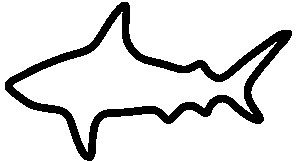
\includegraphics[width=4.5cm]{sharc_logo.png}};


%%%% SPaiNN
\draw[draw=black!40!ocp, fill=black!30!ocp, line width=0.75pt] (5.5,2.9) rectangle node[font=\sansmath\sffamily\small, white, bag, rotate=90]{$\mathbf{ML~model}$} (6.0,1.1);

\node[anchor=west, font=\sansmath\sffamily\small, HH] at (5.35,0.6) {\textbf{\textsc{SPaiNNulator}}};
\node[anchor=west, font=\sansmath\sffamily\small, black!30!gray] at (9.6,0.4) {\textbf{\textsc{SHARC}}};

\node[anchor=west, font=\sansmath\sffamily\small, black!30!ocp, rotate=90] at (5.25,1.2) {\textbf{\textsc{SchNetPack}}};

%%%%% SHARC

\draw[fill=black!60!white, draw=none, rounded corners=1pt] (6.9,2.9) rectangle (11.7,2.4);
\node[anchor=west, font=\sansmath\sffamily\scriptsize, white] at (10.9,2.65) {$t$};

\node[anchor=west, font=\sansmath\sffamily\scriptsize, fill=black!30!white, draw=none, rounded corners=1pt] at (8.0-1.0,2.65) {$\mathsf{\vphantom{\nabla_{R}}}R, Z$};
\node[anchor=west, font=\sansmath\sffamily\scriptsize, fill=white!30!sii, draw=none, rounded corners=1pt] at (8.97-1.0,2.65) {$\nabla_R E_j$};
\node[anchor=west, font=\sansmath\sffamily\scriptsize, fill=white!30!sii, draw=none, rounded corners=1pt] at (9.85-1.0,2.65) {$\vphantom{\mathsf{\mathbf{\nabla_{R}}}E_j}C_{ji}, H_{ji}$};
\node[anchor=west, font=\sansmath\sffamily\scriptsize, fill=white!30!sii, draw=none, rounded corners=1pt] at (10.82-1.0,2.65) {$\vphantom{\mathsf{\mathbf{\nabla_{R}}}E_j}c_j$};
\node[anchor=west, font=\sansmath\sffamily\scriptsize, fill=white!30!sii, draw=none, rounded corners=1pt] at (11.32-1.0,2.65) {$\vphantom{\mathsf{\mathbf{\nabla_{R}}}E_j}\mathsf{j}$};

\draw[fill=black!30!white, draw=none, rounded corners=1pt] (6.9,1.6) rectangle (11.7,1.1);
\node[anchor=west, font=\sansmath\sffamily\scriptsize, white] at (10.9,1.35) {$t + \Delta{}t$};

\node[anchor=west, font=\sansmath\sffamily\scriptsize, fill=black!70!white, draw=none, rounded corners=1pt] at (8.0-1.0,1.35) {\textcolor{white}{$\mathsf{\vphantom{\nabla_{R}}}R, Z$}};
\node[anchor=west, font=\sansmath\sffamily\scriptsize, fill=black!50!sii, draw=none, rounded corners=1pt] at (8.97-1.0,1.35) {\textcolor{white}{$\nabla_R E_j$}};
\node[anchor=west, font=\sansmath\sffamily\scriptsize, fill=black!50!sii, draw=none, rounded corners=1pt] at (9.85-1.0,1.35) {\textcolor{white}{$\vphantom{\mathsf{\mathbf{\nabla_{R}}}E_j}C_{ji}, H_{ji}$}};
\node[anchor=west, font=\sansmath\sffamily\scriptsize, fill=black!50!sii, draw=none, rounded corners=1pt] at (10.82-1.0,1.35) {\textcolor{white}{$\vphantom{\mathsf{\mathbf{\nabla_{R}}}E_j}c_j$}};
\node[anchor=west, font=\sansmath\sffamily\scriptsize, fill=black!50!sii, draw=none, rounded corners=1pt] at (11.32-1.0,1.35) {\textcolor{white}{$\vphantom{\mathsf{\mathbf{\nabla_{R}}}E_j}\mathsf{j}$}};

%%% step 1

\draw[HH, line width=1.0pt, rounded corners, smooth, line cap=round, ->] (7.0,2.65) to node[font=\sansmath\sffamily\scriptsize, above, yshift=-0.2mm]{\circled{$\mathsf{1}$}} (6.0,2.65);

\draw[HH, line width=1pt, rounded corners, smooth, line cap=round, ->] (5.75, 2.9) to (5.75,3.10) to (8.35,3.10) to (8.35,2.85);
\draw[HH, line width=1pt, rounded corners, smooth, line cap=round, ->] (7.5,3.10) to (9.25,3.10) to (9.25,2.85);

%%% step 2

\draw[black!30!gray, line width=0.8pt, rounded corners, smooth, line cap=round, ->] (7.3,2.43) to (7.3,1.55);
\draw[black!30!gray, line width=0.8pt, rounded corners, smooth, line cap=round, ->] (8.35,2.43) to (8.35,2.15) to node[font=\sansmath\sffamily\scriptsize, below, yshift=-0.05mm]{\circled{$\mathsf{2}$}}  (7.3,2.15) to (7.3,1.55);

%%% step 3

\draw[HH, line width=1pt, rounded corners, smooth, line cap=round, ->] (7.0,1.35) to node[font=\sansmath\sffamily\scriptsize, below, yshift=0.2mm]{\circled{$\mathsf{3}$}} (6.0,1.35);

\draw[HH, line width=1pt, rounded corners, smooth, line cap=round, ->] (5.75, 1.1) to (5.75,0.90) to (8.20,0.90) to (8.20,1.15);
\draw[HH, line width=1pt, rounded corners, smooth, line cap=round, ->] (5.75, 1.1) to (5.75,0.90) to (9.25,0.90) to (9.25,1.15);

%%% step 4

\draw[black!30!gray, line width=0.8pt, rounded corners, smooth, line cap=round, ->] (9.95,2.43) to (9.95,1.55);
\draw[black!30!gray, line width=0.8pt, rounded corners, smooth, line cap=round, ->] (9.25,2.43) to (9.25,2.15) to (9.95,2.15) to (9.95, 1.55);
\draw[black!30!gray, line width=0.8pt, rounded corners, smooth, line cap=round, ->] (9.25,1.55) to (9.25,2.15) to node[font=\sansmath\sffamily\scriptsize, below, yshift=-0.05mm]{\circled{$\mathsf{4}$}} (9.95,2.15) to (9.95, 1.55);

%%% step 5

\node[anchor=west, font=\sansmath\sffamily\scriptsize, fill=black!50!theo, draw=none, rounded corners=1pt] at (10.7,2.1) {\textcolor{white}{$h$}};

\draw[black!30!gray, line width=0.8pt, rounded corners, smooth, line cap=round, ->] (10.05,2.43) to (10.05,2.15) to (10.7, 2.15);
\draw[black!30!gray, line width=0.8pt, rounded corners, smooth, line cap=round, ->] (10.45,2.43) to (10.45,2.15) to (10.7, 2.15);
\draw[black!30!gray, line width=0.8pt, rounded corners, smooth, line cap=round, ->] (10.7,2.05) to (10.45,2.05) to node[font=\sansmath\sffamily\scriptsize, left, yshift=1.1mm]{\circled{$\mathsf{5}$}} (10.45, 1.55);

%%% step 6

\draw[black!30!gray, line width=0.8pt, rounded corners, smooth, line cap=round, ->] (10.45,1.15) to (10.45,0.70) to node[font=\sansmath\sffamily\scriptsize, above, xshift=5mm, yshift=-0.3mm]{\circled{$\mathsf{6}$}} (8.45, 0.7) to (8.45,1.15);
\draw[black!30!gray, line width=0.8pt, rounded corners, smooth, line cap=round, ->] (7.3,1.15) to (7.3,0.70) to (8.45,0.70) to (8.45,1.15);




\end{tikzpicture} 
\end{document}

